\chapter{Deep Learning}
\label{sec:deep_learning}

This chapter provides all the background required to understand, reproduce, and critically analyze the deep learning tools employed throughout this thesis. Owing to the versatility of deep learning models and their capacity to approximate complex, high-dimensional mappings, these methods offer a powerful framework for addressing challenging problems in Physics and Mathematics.

By introducing the essential concepts needed to formulate, train, test, and analyze deep learning models, this chapter establishes the foundations for constructing architectures tailored to specific physical constraints and learning objectives. In particular, such models enable the treatment of problems that are otherwise computationally prohibitive using conventional numerical methods, including the quantum marginal problem discussed in the previous chapter and the simulation of complex quantum dynamics with reduced computational resources.

Given the broad scope of Deep Learning as a research field, the discussion in this chapter is intentionally limited to the concepts and techniques that are directly relevant to the developments presented in this thesis. Throughout this chapter, the references \cite{Goodfellow2016, Neuer2021} are adopted as the primary sources for the theoretical and methodological aspects of deep learning.

% ============================================================
\section{Motivation and scope}
\label{sec:dl_motivation}

Deep learning has demonstrated remarkable versatility across a wide range of disciplines, spanning from large-scale commercial applications to advanced scientific research. In many contexts, deep learning models have outperformed traditional numerical and algorithmic approaches when dealing with high-dimensional, nonlinear, or poorly structured problems. This capability has enabled the development of practical solutions to tasks that, prior to the emergence of modern deep learning techniques, were widely regarded as computationally infeasible or even impossible.

As mentioned in the Introduction, deep learning has been successfully applied to a variety of problems, including image and signal processing, natural language modeling, and the approximation of complex dynamical systems. Beyond their empirical success, these models provide a flexible mathematical framework for learning representations and mappings directly from data, without requiring explicit handcrafted features or closed-form analytical models.

Despite their empirical success, deep learning models are often informally referred to as \textit{black-box} models. This characterization reflects the perceived opacity of their internal mechanisms rather than a lack of underlying mathematical structure. However, several authors argue that this description is imprecise, and that deep learning models are more appropriately described as \textit{grey-box} models. Although such models may involve a large number of parameters, their internal operations remain partially traceable and analyzable, which contradicts a strictly black-box interpretation.

In this chapter, we aim to clarify how these models operate internally by introducing the key principles governing their architecture, training, and optimization. This perspective is particularly relevant in physics-based applications, where interpretability, consistency with known physical laws, and controlled generalization play a central role.

% ============================================================
\section{Machine Learning models}
\label{sec:ml_models}

Since Deep Learning is a subfield of Machine Learning, many of the concepts employed in this area originate from the broader Machine Learning framework. In both Machine Learning and Deep Learning, the central objective is to construct algorithms that are able to learn from data rather than being explicitly programmed through fixed rules.

This naturally leads to a fundamental question: what does it mean for a model to \emph{learn}? A widely accepted and operational definition is provided in Ref.~\cite{Goodfellow2016}, which states that
\begin{quote}
    A computer program is said to learn from experience $E$ with respect to some class of tasks $T$ and performance measure $P$, if its performance at tasks in $T$, as measured by $P$, improves with experience $E$.
\end{quote}

This definition highlights three essential components of any learning system: the task $T$ to be performed, the experience $E$ from which the system learns, and the performance measure $P$ used to evaluate its success. Together, these elements provide a precise and practical framework for formulating learning problems in a mathematically and computationally well-defined manner.

In the following sections, we analyze these components in the context of deep learning models and introduce the key elements required to understand neural network architectures, training procedures, and evaluation strategies. This establishes the foundation necessary to construct and analyze learning-based models capable of addressing the complex physical and mathematical problems considered in this thesis.

\paragraph{The task, $T$.}
In Machine Learning, the task $T$ specifies the type of problem that the algorithm is designed to solve and determines how input data are processed to produce meaningful outputs. Data are typically represented as collections of features extracted or measured from a physical, mathematical, or computational system, and the task defines the mapping that the model is expected to learn from these features.

A wide variety of tasks can be addressed within this framework. Common examples include classification, where the objective is to assign discrete labels to inputs; regression, which aims to predict continuous-valued outputs; transcription and representation learning, where data are mapped into alternative representations; anomaly detection, which focuses on identifying atypical patterns; interpolation and denoising tasks; and probability density estimation. The specific choice of the task $T$ is dictated by the nature of the problem under study and by the type of information one aims to extract from the data.

\paragraph{The experience, $E$.}
The experience $E$ refers to the data from which the learning algorithm acquires information. A useful distinction arises when categorizing Machine Learning approaches according to the type of experience provided during training.

In \emph{supervised} learning, the experience consists of labeled data pairs, typically of the form $(\mathbf{x}, \mathbf{y})$, where $\mathbf{x}$ denotes the input features and $\mathbf{y}$ represents the desired output. The learning process aims to infer a functional relationship that maps inputs to outputs by minimizing a discrepancy between model predictions and known targets.

In contrast, \emph{unsupervised} learning relies on unlabeled data, where only the input samples $\mathbf{x}$ are available. In this case, the objective is to uncover hidden structures, correlations, or representations intrinsic to the data itself, without explicit target values. Both paradigms play an important role in Deep Learning, depending on the availability of data and the nature of the task being addressed.

\paragraph{The performance measure, $P$.}
The performance measure $P$ quantifies how well a learning algorithm performs the assigned task and plays a central role during the training stage. Since learning-based models aim to approximate an unknown mapping from data, discrepancies between model predictions and observed values naturally arise. The purpose of the performance measure is to provide a scalar quantity that evaluates these discrepancies and allows different candidate models to be compared.

There exists considerable flexibility in the choice of performance measures, depending on the task under consideration. In regression problems, a common choice is to evaluate the deviation between predicted and measured values through an averaged error criterion.

To illustrate this idea, consider the simple example of \emph{linear regression}. Given a set of measured data points $\{(x_i, y_i)\}_{i=1}^N$, the task consists of finding a linear function
\begin{equation}
    y(x) = m x + n,
\end{equation}
that best describes the relationship between the variables $x$ and $y$. Although two exact data points are sufficient to determine a unique linear function in an ideal noiseless setting, real measurements are typically affected by noise. As a consequence, infinitely many linear functions may be compatible with the data within experimental uncertainty.

To compare different candidate functions, a performance function can be introduced. For instance, one may define
\begin{equation}
    \mathcal{L}(m,n) =
    \frac{1}{N} \sum_{i=1}^{N}
    \qty( m x_i + n - y_i )^2 ,
\end{equation}
which quantifies the average squared deviation between the model predictions and the observed data.

In this example, the three elements of learning are clearly identified: the task $T$ is to approximate the functional relationship between two variables, the experience $E$ is given by the measured data points $(x_i, y_i)$, and the performance measure $P$ provides a quantitative criterion to assess how well the model performs the task.


% ============================================================
\section{Artificial neural networks}
\label{sec:neural_networks}

A central pillar of this thesis is the use of artificial neural networks (ANNs). In this work, they are employed to construct models—i.e., computer programs—designed to accomplish the tasks T previously introduced. An artificial neural network is built from basic computational units commonly referred to as neurons or perceptrons, which constitute the fundamental elements of these architectures.

The terminology neuron originates from the fact that neural networks were originally inspired by the interconnected structure of biological neural systems, such as those found in the human brain. However, despite this inspiration, artificial neural networks do not operate according to the same principles as biological neural systems and exhibit substantial differences in their underlying mechanisms \cite{Bowers2023}.

Nevertheless, the computational behavior of artificial perceptrons is sufficient to construct robust and versatile models that have proven effective across a wide range of tasks. In this thesis, some of these tasks that can be successfully addressed using artificial neural networks are explored and analyzed.

\paragraph{Artificial neurons}
The basic structure of an artificial neuron can be conveniently described using linear algebra. Let
$\mathbf{x} = (x_1, \dots, x_n) \in \mathbb{R}^n$
denote the input vector of the neuron, and
$\boldsymbol{\omega} = (\omega_1, \dots, \omega_n)$
the corresponding vector of trainable weights. The neuron computes an affine transformation of the input followed by a nonlinear activation function $f$, yielding the output
\begin{equation}
    \label{eq:single-neuron}
    y = f \qty( \boldsymbol{\omega} \cdot \mathbf{x} + b ).
\end{equation}

The bias parameter $b$ allows the activation function to be shifted independently of the input, thereby increasing the expressive capacity of the neuron. For a fixed activation function, the response of the neuron is entirely determined by the values of the weights and the bias, which are adjusted during training in order to satisfy the requirements of the target task.

\paragraph{Forward propagation}
Once the functioning of a single perceptron is understood, it is natural to extend the construction to a collection of perceptrons arranged in layers, forming a neural network capable of processing data. Consider a layer composed of $k$ artificial neurons. The output of the $i$-th neuron in this layer is given by
\begin{equation}
    \label{eq:layer_1}
    y^{(k)}_i = f\qty( \boldsymbol{\omega}^{(k)}_i \cdot \mathbf{x} + b^{(k)}_i ),
\end{equation}
where $\boldsymbol{\omega}^{(k)}_i$ and $b^{(k)}_i$ denote the weights and bias associated with the $i$-th neuron of the layer, respectively, and $f$ is the activation function applied element-wise.

Subsequently, additional layers can be stacked on top of the first one. For instance, if the input to the second layer is given by the output vector of the first layer, $\mathbf{y}_1 = (y^{(k)}_1,\dots,y^{(k)}_k)$, then the output of the $j$-th neuron in the second layer is
\begin{equation}
    y^{(k)}_{2,j} = g \qty( \boldsymbol{\omega}^{(k)}_{2,j} \cdot \mathbf{y}_1 + b^{(k)}_{2,j} ),
\end{equation}
where $\boldsymbol{\omega}^{(k)}_{2,j}$ and $b^{(k)}_{2,j}$ are the weights and bias of the corresponding neuron in the second layer. The activation function $g$ may differ from $f$, although in practice it is common—but not mandatory—to use the same activation across multiple layers.

This construction can be generalized to a neural network composed of $L$ layers, where each layer introduces additional weights and biases, increasing the number of free parameters available for optimization during training. These parameters are adjusted in order to approximate a target mapping associated with a given task. In this context, the matrix representation of the neural network can be written in a compact form. Let $\mathbf{a}^{(0)} \equiv \mathbf{x}$ denote the input vector, and consider the $l$-th layer characterized by a weight matrix $\mathbf{W}^{(l)} \in \mathbb{R}^{n_l \times n_{l-1}}$, a bias vector $\mathbf{b}^{(l)} \in \mathbb{R}^{n_l}$, and an activation function $\sigma^{(l)}(\cdot)$. The forward propagation through the network is then given by
\begin{equation}
    \label{eq:fully-connected-network}
    \mathbf{a}^{(l)} = \sigma^{(l)}\!\left( \mathbf{W}^{(l)} \mathbf{a}^{(l-1)} + \mathbf{b}^{(l)} \right),
\end{equation}
where the activation function is applied element-wise. The output of the network corresponds to $\mathbf{y} = \mathbf{a}^{(L)}$, with $L$ denoting the total number of layers. A similar description can be found in Ref.~\cite{Lu2021}, where the authors develop a Python-based framework to solve differential equations using this class of neural networks. This application will be discussed later in this chapter.

Models of this type are referred to as \emph{feedforward} (or \emph{forward}) neural networks, since the output is obtained through a forward propagation of information from the input layer, across successive hidden layers, up to the final output layer. In particular, there exist multiple ways to connect the internal neurons within a neural network. The configuration presented in the Figure~\ref{fig:fully-connected-network} corresponds to the so-called \emph{fully connected} architecture, in which each perceptron in a given layer is connected to every perceptron in the preceding and subsequent layers.
\begin{figure}[ht]
    \centering
    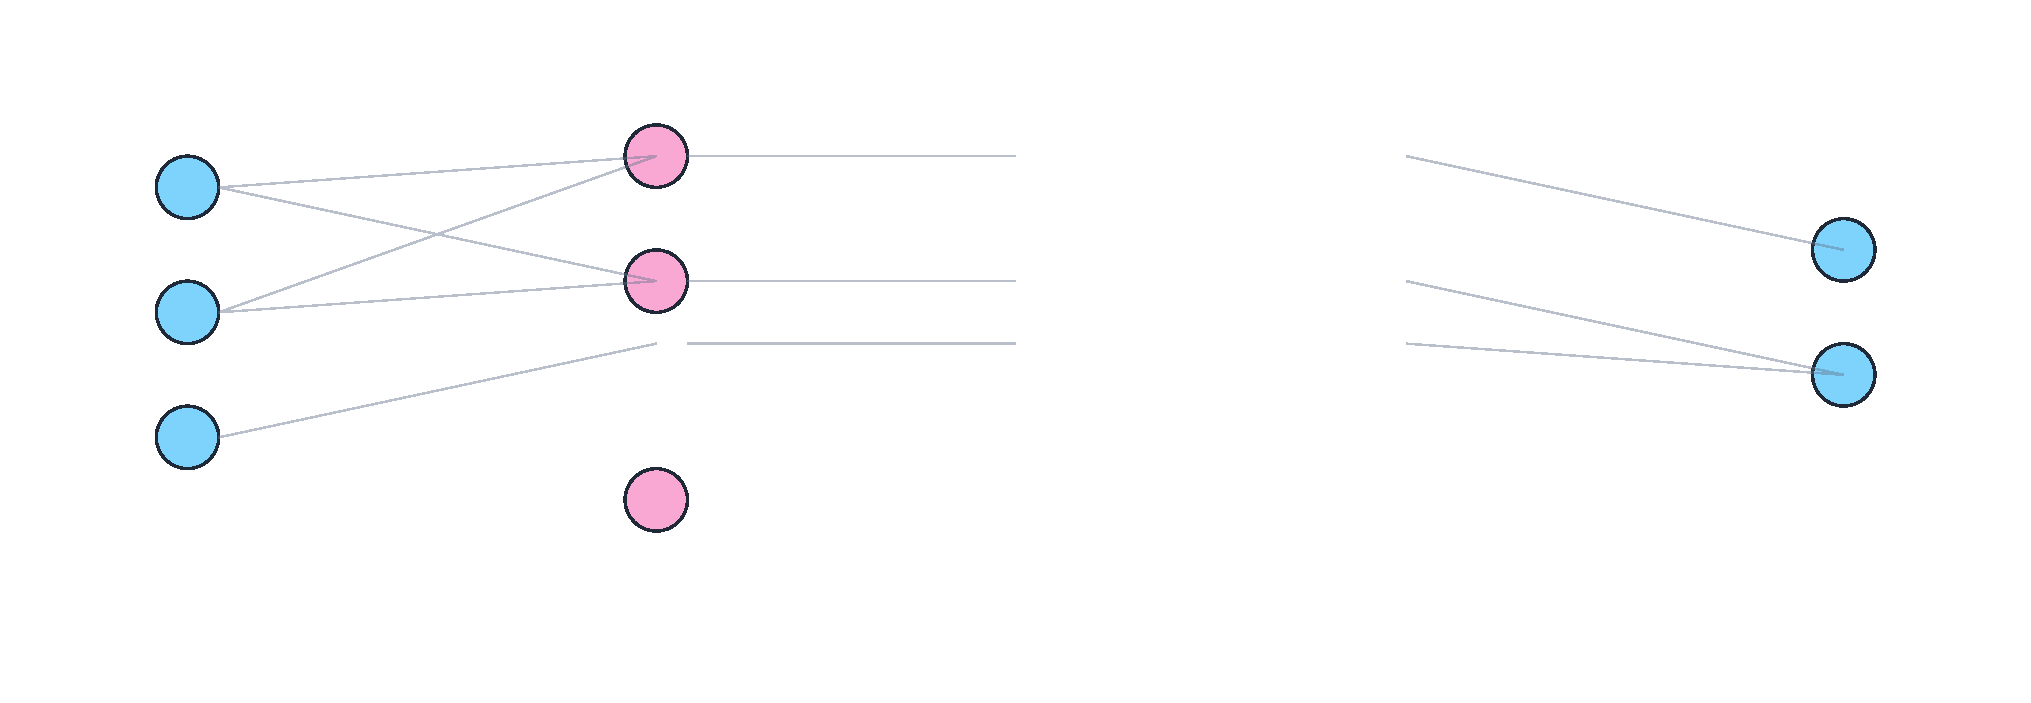
\includegraphics[width=0.9\linewidth]{images/fully-connected.pdf}
    \caption[Deep feedforward neural network]{Schematic representation of a deep feedforward neural network.}
    \label{fig:fully-connected-network}
\end{figure}

In general, while the structure of the input and output layers is strongly dictated by the specific task for which the network is designed, the internal layers—commonly referred to as \emph{hidden layers}—may vary in their connectivity patterns and may incorporate additional mathematical regularization mechanisms, such as batch normalization or dropout. These techniques are task-dependent and implementation-specific; therefore, they are not considered in the present work. We refer to the specific choice of layer organization, connectivity, and associated transformations as the \emph{network architecture}.

\paragraph{Convolutional layers}
The fully connected architecture described previously provides a general framework for constructing neural networks; however, it does not explicitly exploit any structure present in the input data. In many applications, particularly those involving spatially distributed data such as images, grids, or discretized physical fields, the input exhibits strong local correlations. In such cases, fully connected layers become parameter-inefficient and may fail to capture relevant inductive biases due to the large number of free parameters (weights and biases). Convolutional layers address this limitation by introducing structured weight sharing through the convolution operation. Instead of learning an independent weight for each input--output connection, a convolutional layer applies a set of local kernels across the input domain, enforcing translational equivariance and significantly reducing the number of trainable parameters.

A defining characteristic of convolutional layers is the use of shared weights. In contrast to fully connected layers, where each connection between neurons is associated with an independent weight, convolutional layers employ the same kernel parameters across all spatial locations of the input. As a consequence, a single kernel captures repeated local patterns throughout the entire domain, and its parameters are optimized collectively based on their global contribution to the network output.

The convolution operation for continuous functions can be written as
\begin{equation}
    s(t) = (x * \omega)(t) = \int x(a)\,\omega(t - a)\,\mathrm{d}a,
\end{equation}
where the symbol $*$ denotes convolution, $x$ represents the input function, and $\omega$ is a weight function.

In the context of neural networks, $x$ is interpreted as the \emph{input} of the layer, while the weight function $\omega$ is referred to as the \emph{kernel}. The output of the convolutional layer is commonly called the \emph{feature map}. Although convolution is naturally defined for continuous functions, machine learning applications typically employ a discrete formulation, given by
\begin{equation}
    s(t) = (x * \omega)(t) = \sum_{a=-\infty}^{\infty} x(a)\,\omega(t - a),
\end{equation}
where $a$ is an integer-valued variable indexing the input domain.

In practical applications, the input is usually a multidimensional array and the kernel is a multidimensional tensor of trainable parameters. For example, considering a two-dimensional input such as an image, the convolution operation takes the form
\begin{equation}
    S(i,j) = (I * K)(i,j) = \sum_{m,n} I(m,n)\,K(i - m, j - n),
\end{equation}
where $I$ denotes the input array, $K$ the kernel, and $(i,j)$ label spatial coordinates.

The forward propagation through a convolutional layer can therefore be expressed as
\begin{equation}
    \mathbf{a}^{(l)} =
    \sigma^{(l)}\!\left(
    \mathbf{K}^{(l)} * \mathbf{a}^{(l-1)} + \mathbf{b}^{(l)}
    \right),
\end{equation}
where $\mathbf{K}^{(l)}$ denotes the convolutional kernel tensor, $\mathbf{b}^{(l)}$ is the bias term, $*$ represents the discrete convolution operator, and $\sigma^{(l)}$ is applied element-wise.

Beyond the kernel itself, the behavior of a convolutional layer is governed by several structural hyperparameters. The \emph{stride} controls the displacement of the kernel between successive applications, with larger strides reducing the spatial resolution of the resulting feature maps. The \emph{padding} operation extends the input domain, commonly by adding zeros, allowing control over output dimensions and mitigating boundary effects. The \emph{dilation} parameter introduces spacing between kernel elements, effectively increasing the receptive field without increasing the number of parameters. Finally, the \emph{groups} parameter partitions the input channels into independent subsets, enabling grouped or depth-wise convolutions and reducing computational complexity.

Figure~\ref{fig:conv-connected-network} illustrates a comparison between fully connected layers and convolutional layers in terms of the number of internal connections, that is, the number of free parameters. By restricting each neuron to interact only with a local neighborhood of the input, convolutional layers drastically reduce the number of trainable parameters. As a consequence, the values of the weights are determined by local correlations in the data, leading to a significant reduction in computational cost while preserving the ability to extract relevant features.

\begin{figure}[ht]
    \centering
    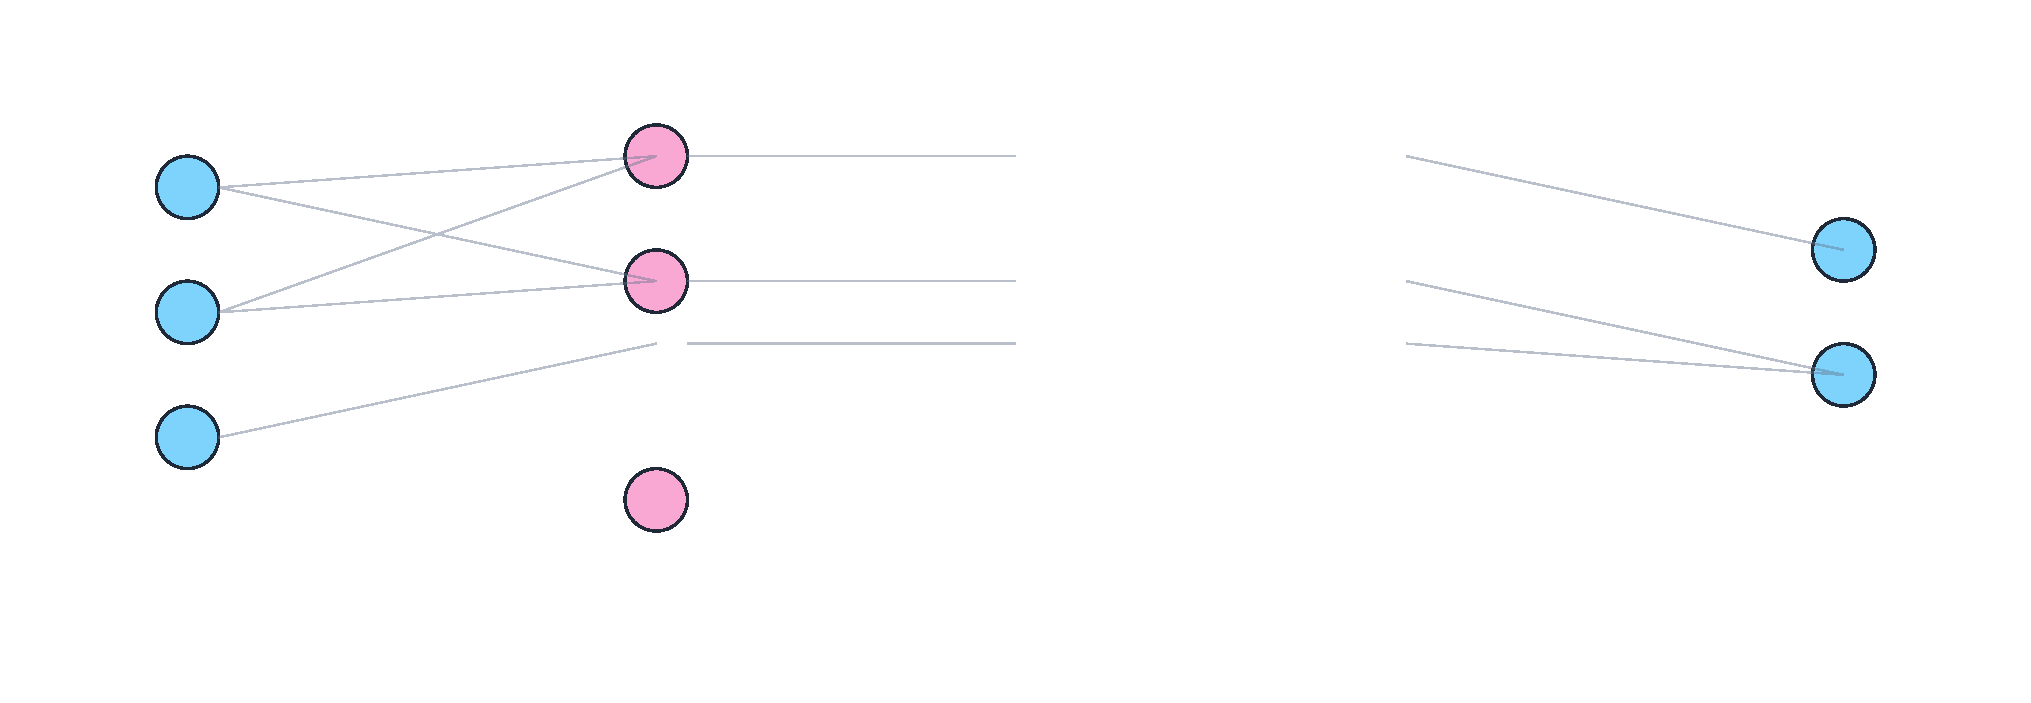
\includegraphics[width=0.9\linewidth]{images/conv-connected.pdf}
    \caption[Neural network made by CNN's and fully connected layers]{Schematic representation of a deep feedforward neural network combining convolutional and fully connected layers.}
    \label{fig:conv-connected-network}
\end{figure}

% ============================================================
\section{Activation functions}
\label{sec:activation_functions}

One of the key components of Artificial Neural Networks (ANNs) is the activation function. Its role is to introduce non-linearity into the model, allowing the network to represent complex relationships beyond linear mappings. In practice, the activation function determines how the weighted input of a neuron is transformed before being propagated to subsequent layers, effectively controlling whether and how a neuron contributes to the overall network output.

Several activation functions have been proposed in the literature. Among the most commonly used ones is the hyperbolic tangent function ($\tanh$), which maps the input to a bounded interval $(-1,1)$ and is often preferred in physical and dynamical contexts due to its smoothness and symmetry around zero. Another widely used activation function is the sigmoid function, which produces outputs in the interval $(0,1)$ and has historically been employed in early neural network models, particularly in probabilistic interpretations. More recently, the Rectified Linear Unit (ReLU) has become popular due to its computational simplicity and its ability to alleviate vanishing gradient effects in deeper architectures.

The choice of activation function directly impacts the expressive power, numerical stability, and trainability of the network, and therefore constitutes an important design consideration in neural network models. Figure~\ref{fig:activation} illustrates several commonly used activation functions.

\begin{figure}[ht]
    \centering
    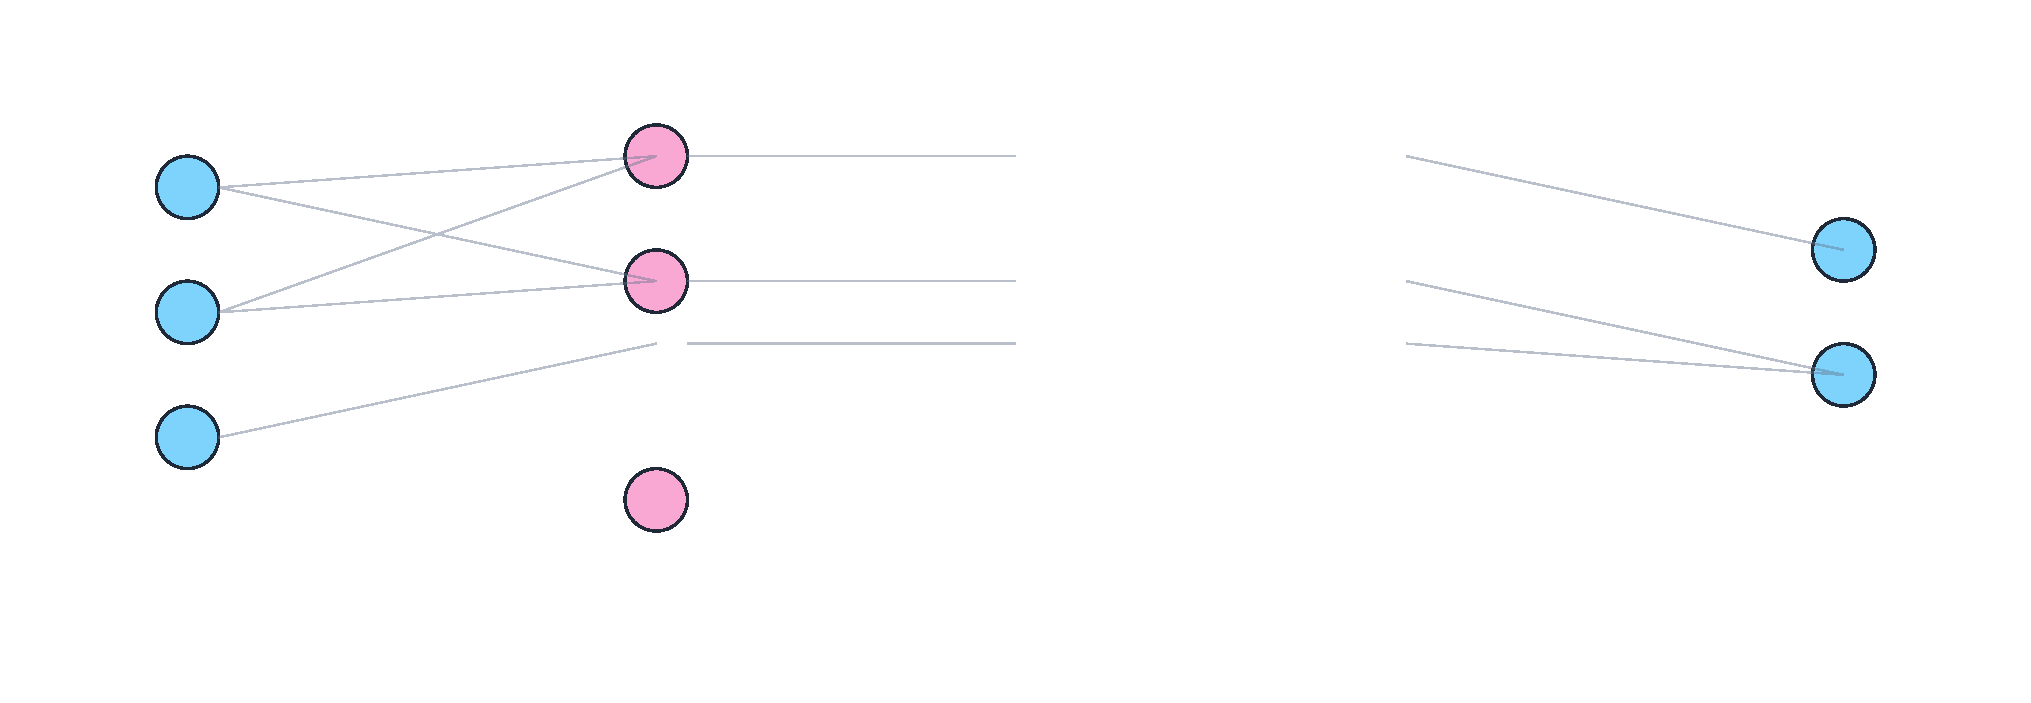
\includegraphics[width=0.9\linewidth]{images/activation-func.pdf}
    \caption[Activation functions]{Examples of commonly used activation functions, including $\tanh$, sigmoid, and ReLU.}
    \label{fig:activation}
\end{figure}

\section{Loss functions and training objective} 
\label{sec:loss_functions}

The versatility of Deep Learning models stems from the wide range of tasks that can be addressed using them, some of which were outlined in the Introduction. However, one of the most crucial aspects of these models is not the architectures themselves, but rather the procedures employed to train them for a specific task. At a conceptual level, training is based on comparing the model output with a reference dataset and iteratively adjusting the internal parameters of the model in order to minimize this discrepancy.

More precisely, the training process relies on the definition of a scalar function that quantifies the disagreement between the model prediction and the target data. Let $\mathcal{L}$ denote such a function, defined here as the squared distance between the network output $\mathbf{y}_{\mathrm{net}}$ and the reference data $\mathbf{d}$,
\begin{equation}
    \label{eq:loss-example}
    \mathcal{L} = \sum_i \qty( y_i - d_i )^2 .
\end{equation}

This quantity is commonly referred to as the \emph{loss function} or \emph{cost function}. When the internal parameters of the model are appropriately chosen, the value of $\mathcal{L}$ approaches zero, indicating that the model successfully reproduces the target data $\mathbf{d}$ and, consequently, performs the desired task.

For illustrative purposes, consider a model composed of a single fully connected layer. In this case, the trainable parameters correspond to the weights and biases of the perceptrons. For an input vector $\mathbf{x} = (x_1,\dots,x_n)$, the pre-activation variable associated with the $i$-th neuron is given by
\begin{equation}
    z_i = \sum_j W_{ij} x_j + b_i ,
\end{equation}
and the corresponding network output is
\begin{equation}
    y_i = \sigma(z_i),
\end{equation}
where $\sigma(\cdot)$ denotes the activation function. The loss function in Eq.~\eqref{eq:loss-example} can then be written as
\begin{equation}
    \mathcal{L} = \sum_i \qty( \sigma\qty( \sum_j W_{ij} x_j + b_i ) - d_i )^2 .
\end{equation}

The optimization of the model parameters is carried out by evaluating the partial derivatives of the loss function with respect to each trainable parameter. Since each neuron $i$ is associated with a set of weights $W_{ij}$, the gradient of the loss function is naturally expressed using two indices. Applying the chain rule, the partial derivative of $\mathcal{L}$ with respect to a weight parameter $W_{ij}$ reads
\begin{equation}
    \pdv{\mathcal{L}}{W_{ij}}
    =
    \pdv{\mathcal{L}}{y_i}
    \pdv{y_i}{z_i}
    \pdv{z_i}{W_{ij}} .
\end{equation}

This expression quantifies how variations in a specific weight $W_{ij}$ affect the model performance and forms the basis of gradient-based optimization algorithms employed during the training process. The central idea is to iteratively update the weights in the direction of the negative gradient, thereby minimizing the value of the loss function $\mathcal{L}$. This procedure is commonly referred to as the \emph{gradient descent} method.

When the model consists of more than a single layer, the computation of the gradients must be performed sequentially, starting from the output layer and propagating backwards through the network. This process, well established in the literature, is known as \emph{backpropagation}. It constitutes one of the central pillars of Deep Learning and enables the efficient training of neural networks containing millions of parameters.

For a fully connected neural network composed of $L$ layers, the forward propagation can be written in a compact form as shown in Eq.~\eqref{eq:fully-connected-network}. Within this formulation, the gradient of the loss function with respect to the parameters of an intermediate layer can be expressed through successive applications of the chain rule. In particular, the gradient of $\mathcal{L}$ with respect to the weight matrix of the $l$-th layer, with $l \in \{1,\dots,L\}$, takes the general form
\begin{equation}
    \pdv{\mathcal{L}}{\mathbf{W}^{(l)}}
    =
    \pdv{\mathcal{L}}{\mathbf{a}^{(L)}}
    \prod_{k=l+1}^{L}
    \pdv{\mathbf{a}^{(k)}}{\mathbf{a}^{(k-1)}}
    \pdv{\mathbf{a}^{(l)}}{\mathbf{W}^{(l)}} ,
\end{equation}
where the explicit structure of each term depends on the network architecture, including the number of layers, the number of neurons per layer, and the choice of activation functions.

Therefore, in practical scenarios, the explicit analytical form of the gradients is not written out in full. Instead, gradient-based optimization relies on algorithmic implementations of backpropagation, which efficiently evaluate these derivatives without requiring their explicit expansion.

It is worth noting that the explicit form of the gradients differs when the network architecture incorporates convolutional layers instead of fully connected ones. In this case, the trainable parameters correspond to convolutional kernels rather than individual weights, and the training objective remains unchanged: to determine how variations in these parameters affect the network output and the value of the loss function. As a consequence of the convolutional structure, the resulting gradients reflect aggregated contributions over the corresponding receptive fields, rather than local derivatives associated with single connections. As in the fully connected case, the explicit analytical expression of these gradients is not of primary relevance at this level of description, since their evaluation is handled by backpropagation algorithms implemented within modern deep learning frameworks. Nevertheless, understanding the general mechanism by which such gradients are computed and propagated remains important for the correct interpretation, design, and application of convolutional architectures.

\paragraph{Examples of common loss functions}
While the squared loss introduced in Eq.~\eqref{eq:loss-example} provides a simple and illustrative example, different tasks often require alternative choices of loss functions. The selection of an appropriate loss function reflects both the nature of the data and the objective of the learning problem, and may significantly influence the training dynamics and the resulting model performance.

For regression tasks, the mean squared error (MSE) is among the most commonly used loss functions, as it directly penalizes deviations between predicted and target values. In classification problems, loss functions such as the binary or categorical cross-entropy are typically employed, as they are better suited to probabilistic interpretations of the network output. Other loss functions, including absolute error measures or task-specific objective functions, may be adopted depending on the desired robustness or structural constraints of the problem.

In physics-based applications, the loss function may further incorporate additional terms encoding prior knowledge or physical constraints, such as conservation laws or differential equations. In such cases, the training objective is no longer solely data-driven but reflects a combination of empirical accuracy and physical consistency. These extended formulations will be discussed in later sections.

% ============================================================
\section{Optimization and training}
\label{sec:optimization}

As discussed previously, neural networks are trained by optimizing a loss function in order to reproduce a set of known data samples. The underlying idea is that, given a sufficiently representative dataset, the model is able to identify relevant patterns such that, after training, it can successfully perform a specific task. From this perspective, the training of a neural network can be naturally interpreted as an optimization problem defined over a high-dimensional parameter space.

A fundamental connection therefore arises between neural networks and optimization theory. The adjustment of the trainable parameters is carried out through backpropagation, which provides the gradients of the loss function with respect to the model parameters. These gradients are then used by optimization algorithms to iteratively update the parameters. Among the most widely used optimization methods are Stochastic Gradient Descent (SGD) and adaptive schemes such as Adam, both of which are employed in the applications presented in this thesis. A comprehensive overview of optimization algorithms commonly used in deep learning can be found in Ref.~\cite{Ruder2016}.

In its general form, gradient-based optimization updates the parameters $\boldsymbol{\theta}$ of the model according to
\begin{equation}
    \boldsymbol{\theta}_{t+1} = \boldsymbol{\theta}_t - \eta \, \nabla_{\boldsymbol{\theta}} \mathcal{L}(\boldsymbol{\theta}_t),
\end{equation}
where $\boldsymbol{\theta}$ denotes the collection of all trainable parameters of the model and $\nabla_{\boldsymbol{\theta}} \mathcal{L}$ represents the vector of partial derivatives of the loss function with respect to each parameter. Explicitly, for a parameter $\theta_k$, this update rule reads
\begin{equation}
    \theta_k^{(t+1)} = \theta_k^{(t)} - \eta \, \pdv{\mathcal{L}}{\theta_k}\Bigg|_{\boldsymbol{\theta} = \boldsymbol{\theta}_t}.
\end{equation}
Here, $\eta > 0$ is the \emph{learning rate}, a hyperparameter that controls the magnitude of the parameter updates. The learning rate plays a central role in the training dynamics: values that are too large may lead to unstable optimization, while excessively small values can result in slow convergence or stagnation.

In practical implementations, the learning rate is often adjusted during training through the use of \emph{learning rate schedulers}, which progressively reduce its value as the optimization proceeds. This strategy allows for larger exploratory steps during the early stages of training, followed by finer adjustments as the loss function approaches a minimum.

Despite the effectiveness of gradient-based methods, the optimization landscape of deep neural networks is typically highly non-convex and may exhibit flat regions or multiple local minima. A well-known challenge in this context is the presence of \emph{barren plateaus}, where the gradients become extremely small, hindering efficient training. Various techniques have been proposed to mitigate these issues, including the introduction of momentum terms, adaptive learning rate methods, and carefully designed initialization strategies. Such approaches aim to improve convergence by enabling the optimizer to escape shallow local minima or flat regions of the loss landscape.

% ============================================================
\section{Physics-Informed Neural Networks}
\label{sec:pinns}

A central component in the development of deep learning models is the training stage. As previously discussed, training corresponds to the process by which the model learns to perform a specific task by adjusting its internal parameters through optimization. In standard data-driven approaches, this learning is achieved by supplying examples to the model and minimizing a loss function that quantifies the discrepancy between the model outputs and the target data. Through this process, neural networks are able to capture complex internal relationships between the variables involved in the task.

However, in physical sciences, the available information is not limited to observational or simulated data alone. Physical systems are also governed by well-established theoretical principles, typically expressed in the form of conservation laws, symmetry constraints, or differential equations. Ignoring this prior knowledge during training leads to models that are purely empirical, often requiring large datasets and offering limited extrapolation capabilities. Physics-informed learning addresses this limitation by explicitly incorporating known physical laws into the training process.

Physics-Informed Neural Networks (PINNs) constitute a class of models in which prior physical information is embedded directly into the learning procedure. This is commonly achieved by augmenting the loss function with additional terms that penalize violations of the governing equations or physical constraints, or by applying mathematical transformations to the network outputs in order to enforce such constraints by construction. As a consequence, the optimization process is guided not only by data fidelity but also by physical consistency.

This strategy offers several practical advantages. By constraining the hypothesis space of the model to physically admissible solutions, PINNs typically require fewer training examples, exhibit improved generalization, and converge faster during optimization. Moreover, the resulting models tend to be more robust to noise and better suited for interpolation and extrapolation tasks within the physically relevant regime.

A widely studied and natural application of PINNs is the solution of partial differential equations, where the neural network is trained to approximate the solution of a differential equation while minimizing the residual of the governing equation at a set of collocation points. This framework has been successfully applied to a broad range of problems in classical mechanics, fluid dynamics, and electromagnetism. Comprehensive discussions and extensions of this methodology can be found in Refs.~\cite{Edward2023, Son2023, Ren2025, Prakash2025, Raissi2019, Lu2021, Neuer2021}.

In this thesis, however, the physics-informed paradigm is employed beyond its conventional role as a differential equation solver. We present two applications in the context of quantum information where physics-informed learning is used to address complex physical and mathematical problems. In both cases, known structural properties of quantum systems are incorporated into the learning process, enabling the construction of models that are not only accurate but also consistent with the underlying quantum dynamics. These examples demonstrate that physics-informed neural networks provide a flexible and powerful framework for integrating deep learning techniques with the fundamental principles of quantum theory.

\paragraph{General formulation of Physics-Informed Neural Networks}
Let $\mathcal{N}_{\boldsymbol{\theta}}(\mathbf{x}, t)$ be a neural network parametrized by $\boldsymbol{\theta}$, intended to approximate the solution $u(\mathbf{x}, t)$ of a physical system governed by a differential equation of the form
\begin{equation}
    \mathcal{D}[u(\mathbf{x}, t)] = 0,
\end{equation}
where $\mathcal{D}$ denotes a (possibly nonlinear) differential operator acting on the solution.

In the physics-informed framework, the neural network output is identified with the trial solution,
\begin{equation}
    u(\mathbf{x}, t) \approx \mathcal{N}_{\boldsymbol{\theta}}(\mathbf{x}, t),
\end{equation}
and automatic differentiation is employed to compute the required spatial and temporal derivatives. The physical consistency of the model is enforced by defining a residual function
\begin{equation}
    \mathcal{R}(\mathbf{x}, t; \boldsymbol{\theta}) := \mathcal{D}[\mathcal{N}_{\boldsymbol{\theta}}(\mathbf{x}, t)].
\end{equation}

The training objective is constructed by minimizing a composite loss function of the form
\begin{equation}
    \mathcal{L} = \mathcal{L}_{\mathrm{data}} + \lambda_{\mathrm{phys}} \, \mathcal{L}_{\mathrm{phys}} + \lambda_{\mathrm{bc}} \, \mathcal{L}_{\mathrm{bc}},
\end{equation}
where $\mathcal{L}_{\mathrm{data}}$ enforces agreement with known data (if available), $\mathcal{L}_{\mathrm{phys}}$ penalizes violations of the governing equations,
\begin{equation}
    \mathcal{L}_{\mathrm{phys}} = \frac{1}{N_r} \sum_{i=1}^{N_r} \left| \mathcal{R}(\mathbf{x}_i, t_i; \boldsymbol{\theta}) \right|^2,
\end{equation}
and $\mathcal{L}_{\mathrm{bc}}$ incorporates boundary and initial conditions. The coefficients $\lambda_{\mathrm{phys}}$ and $\lambda_{\mathrm{bc}}$ control the relative importance of each contribution.

This formulation restricts the hypothesis space of the neural network to functions that are compatible with the known physical laws, effectively embedding prior knowledge into the optimization process.

\paragraph{Illustrative examples: solving differential equations with PINNs}
To illustrate the physics-informed approach, we now consider representative examples where PINNs are employed to solve differential equations of increasing complexity.

\subparagraph{One-dimensional wave equation.}
A standard benchmark problem for PINN is the one-dimensional wave equation,
\begin{equation}
    \frac{\partial^2 u(x,t)}{\partial t^2} = c^2 \frac{\partial^2 u(x,t)}{\partial x^2},
\end{equation}
defined on the spatial domain $x \in [0,1]$ and temporal domain $t \in [0,1]$. 
We consider fixed (Dirichlet) boundary conditions,
\begin{equation}
    u(0,t) = u(1,t) = 0,
\end{equation}
together with the initial conditions
\begin{equation}
    u(x,0) = \sin(\pi x), 
    \qquad 
    \partial_t u(x,0) = 0.
\end{equation}

For the particular choice $c=1$, the analytical solution is given by
\begin{equation}
    u(x,t) = \sin(\pi x)\cos(\pi t).
\end{equation}

Within the PINN framework, a neural network $\mathcal{N}_{\boldsymbol{\theta}}(x,t)$ is used to approximate the displacement field $u(x,t)$. The residual of the wave equation is defined as
\begin{equation}
    \mathcal{R}_{\boldsymbol{\theta}}(x,t)
    =
    \partial_t^2 \mathcal{N}_{\boldsymbol{\theta}}(x,t)
    -
    c^2 \partial_x^2 \mathcal{N}_{\boldsymbol{\theta}}(x,t).
\end{equation}

Let $\{(x_i,t_i)\}_{i=1}^{N_f}$ denote the interior collocation points, 
$\{x_j^{(0)}\}_{j=1}^{N_0}$ the points used to enforce the initial conditions, and 
$\{(x_k^{(b)},t_k^{(b)})\}_{k=1}^{N_b}$ the boundary points. 
The discrete loss function minimized during training is given by

\begin{equation}
\mathcal{L}(\boldsymbol{\theta}) 
=
\frac{1}{N_f} 
\sum_{i=1}^{N_f}
\left|
\mathcal{R}_{\boldsymbol{\theta}}(x_i,t_i)
\right|^2
+
\frac{1}{N_0}
\sum_{j=1}^{N_0}
\left|
\mathcal{N}_{\boldsymbol{\theta}}(x_j^{(0)},0)
-
\sin(\pi x_j^{(0)})
\right|^2
\end{equation}

\begin{equation}
+
\frac{1}{N_0}
\sum_{j=1}^{N_0}
\left|
\partial_t \mathcal{N}_{\boldsymbol{\theta}}(x_j^{(0)},0)
\right|^2
+
\frac{1}{N_b}
\sum_{k=1}^{N_b}
\left|
\mathcal{N}_{\boldsymbol{\theta}}(x_k^{(b)},t_k^{(b)})
\right|^2.
\end{equation}

Figure~\ref{fig:wave-pinn} illustrates the standard evaluation procedure, where the predicted solution surface $\mathcal{N}_{\boldsymbol{\theta}}(x,t)$ is compared with the analytical solution, together with a visualization of the absolute error over the full space--time domain. This combined analysis provides both a quantitative and qualitative assessment of the network's accuracy in capturing the wave dynamics.
\begin{figure}
    \centering
    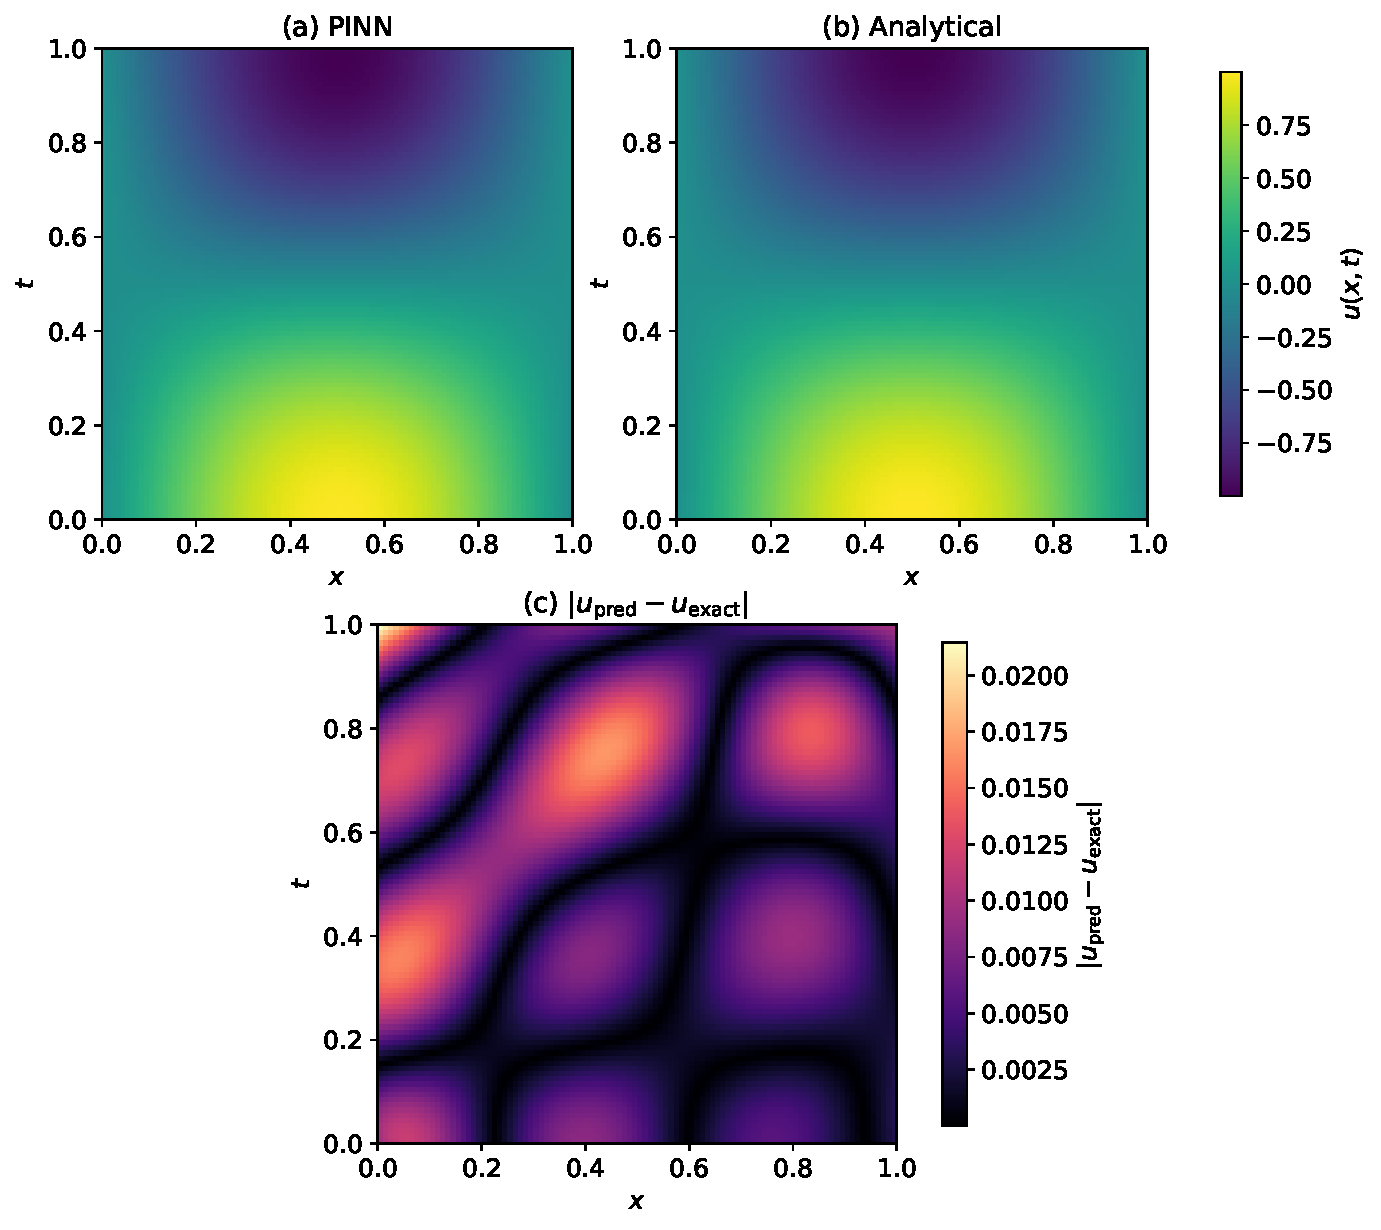
\includegraphics[width=0.95\textwidth]{examples/wave_pinn_comparison.pdf}
    \caption[PINN results for one-dimensional wave equation]{\label{fig:wave-pinn}
    Comparison between the PINN prediction (left), the analytical solution (center), and the absolute error (right). The color scale of the error panel shows that the discrepancy remains uniformly small across the domain, indicating that the network accurately captures both the wave propagation and the imposed boundary conditions.
    }
\end{figure}

\subparagraph{Nonlinear scalar field dynamics.}

As a more complex example, we consider the nonlinear Klein--Gordon equation in $(2+1)$ dimensions,
\begin{equation}
    \frac{\partial^2 \phi(\mathbf{x},t)}{\partial t^2}
    - \nabla^2 \phi(\mathbf{x},t)
    + V'(\phi) = 0,
\end{equation}
where $\mathbf{x} = (x,y)$, $\nabla^2 = \partial_x^2 + \partial_y^2$ denotes the spatial Laplacian, and $V(\phi)$ is a nonlinear potential. 
Such equations arise naturally in classical field theory, high-energy physics, and cosmology, and generally do not admit closed-form analytical solutions when nonlinear interactions are present.

In particular, we consider a quartic self-interaction potential of the form
\begin{equation}
    V(\phi) = \frac{1}{2} m^2 \phi^2 + \frac{\lambda}{4} \phi^4,
\end{equation}
so that
\begin{equation}
    V'(\phi) = m^2 \phi + \lambda \phi^3.
\end{equation}

The resulting evolution equation becomes
\begin{equation}
    \partial_t^2 \phi
    - \partial_x^2 \phi
    - \partial_y^2 \phi
    + m^2 \phi
    + \lambda \phi^3
    = 0.
\end{equation}

The field is defined on a spatial domain $(x,y) \in \Omega \subset \mathbb{R}^2$ and time interval $t \in [0,T]$, supplemented with initial conditions
\begin{equation}
    \phi(x,y,0) = \phi_0(x,y),
    \qquad
    \partial_t \phi(x,y,0) = \pi_0(x,y),
\end{equation}
and suitable boundary conditions (e.g., Dirichlet or periodic).

Within the PINN framework, a neural network $\mathcal{N}_{\boldsymbol{\theta}}(x,y,t)$ is employed to approximate the scalar field $\phi(x,y,t)$. 
A key advantage of PINNs in this context is that the nonlinear interaction term is handled directly through automatic differentiation, without requiring explicit discretization schemes for the spatial derivatives or nonlinear operator.

The corresponding physics residual is defined as
\begin{equation}
    \mathcal{R}_{\boldsymbol{\theta}}(x,y,t)
    =
    \partial_t^2 \mathcal{N}_{\boldsymbol{\theta}}
    -
    \partial_x^2 \mathcal{N}_{\boldsymbol{\theta}}
    -
    \partial_y^2 \mathcal{N}_{\boldsymbol{\theta}}
    +
    m^2 \mathcal{N}_{\boldsymbol{\theta}}
    +
    \lambda \mathcal{N}_{\boldsymbol{\theta}}^3.
\end{equation}

Let $\{(x_i,y_i,t_i)\}_{i=1}^{N_f}$ denote interior collocation points, $\{(x_j^{(0)},y_j^{(0)})\}_{j=1}^{N_0}$ the initial-condition points, and $\{(x_k^{(b)},y_k^{(b)},t_k^{(b)})\}_{k=1}^{N_b}$ boundary points. The discrete loss function minimized during training is given by

\begin{align}
\mathcal{L}(\boldsymbol{\theta})
&=
\frac{1}{N_f}
\sum_{i=1}^{N_f}
\left|
\mathcal{R}_{\boldsymbol{\theta}}(x_i,y_i,t_i)
\right|^2
+
\frac{1}{N_0}
\sum_{j=1}^{N_0}
\left|
\mathcal{N}_{\boldsymbol{\theta}}(x_j^{(0)},y_j^{(0)},0)
-
\phi_0(x_j^{(0)},y_j^{(0)})
\right|^2
\nonumber \\[6pt]
&\quad
+
\frac{1}{N_0}
\sum_{j=1}^{N_0}
\left|
\partial_t \mathcal{N}_{\boldsymbol{\theta}}(x_j^{(0)},y_j^{(0)},0)
-
\pi_0(x_j^{(0)},y_j^{(0)})
\right|^2
+
\frac{1}{N_b}
\sum_{k=1}^{N_b}
\left|
\mathcal{N}_{\boldsymbol{\theta}}(x_k^{(b)},y_k^{(b)},t_k^{(b)})
\right|^2.
\end{align}

Due to the cubic nonlinear term, the dynamics exhibit amplitude-dependent dispersion and nontrivial mode coupling, rendering this problem significantly more challenging than the linear wave equation.

Figure~\ref{fig:field-pinn} displays representative snapshots of the scalar field at different times, while the full dynamical evolution is provided in an accompanying video\footnote{\url{https://youtu.be/bxEir5oOpdk}}. The results reveal a radially propagating structure emerging from the central region. As the field evolves, nonlinear self-interaction induces deformation of the initial profile, generating ring-like wavefronts that expand outward from the origin.

\begin{figure}
    \centering
    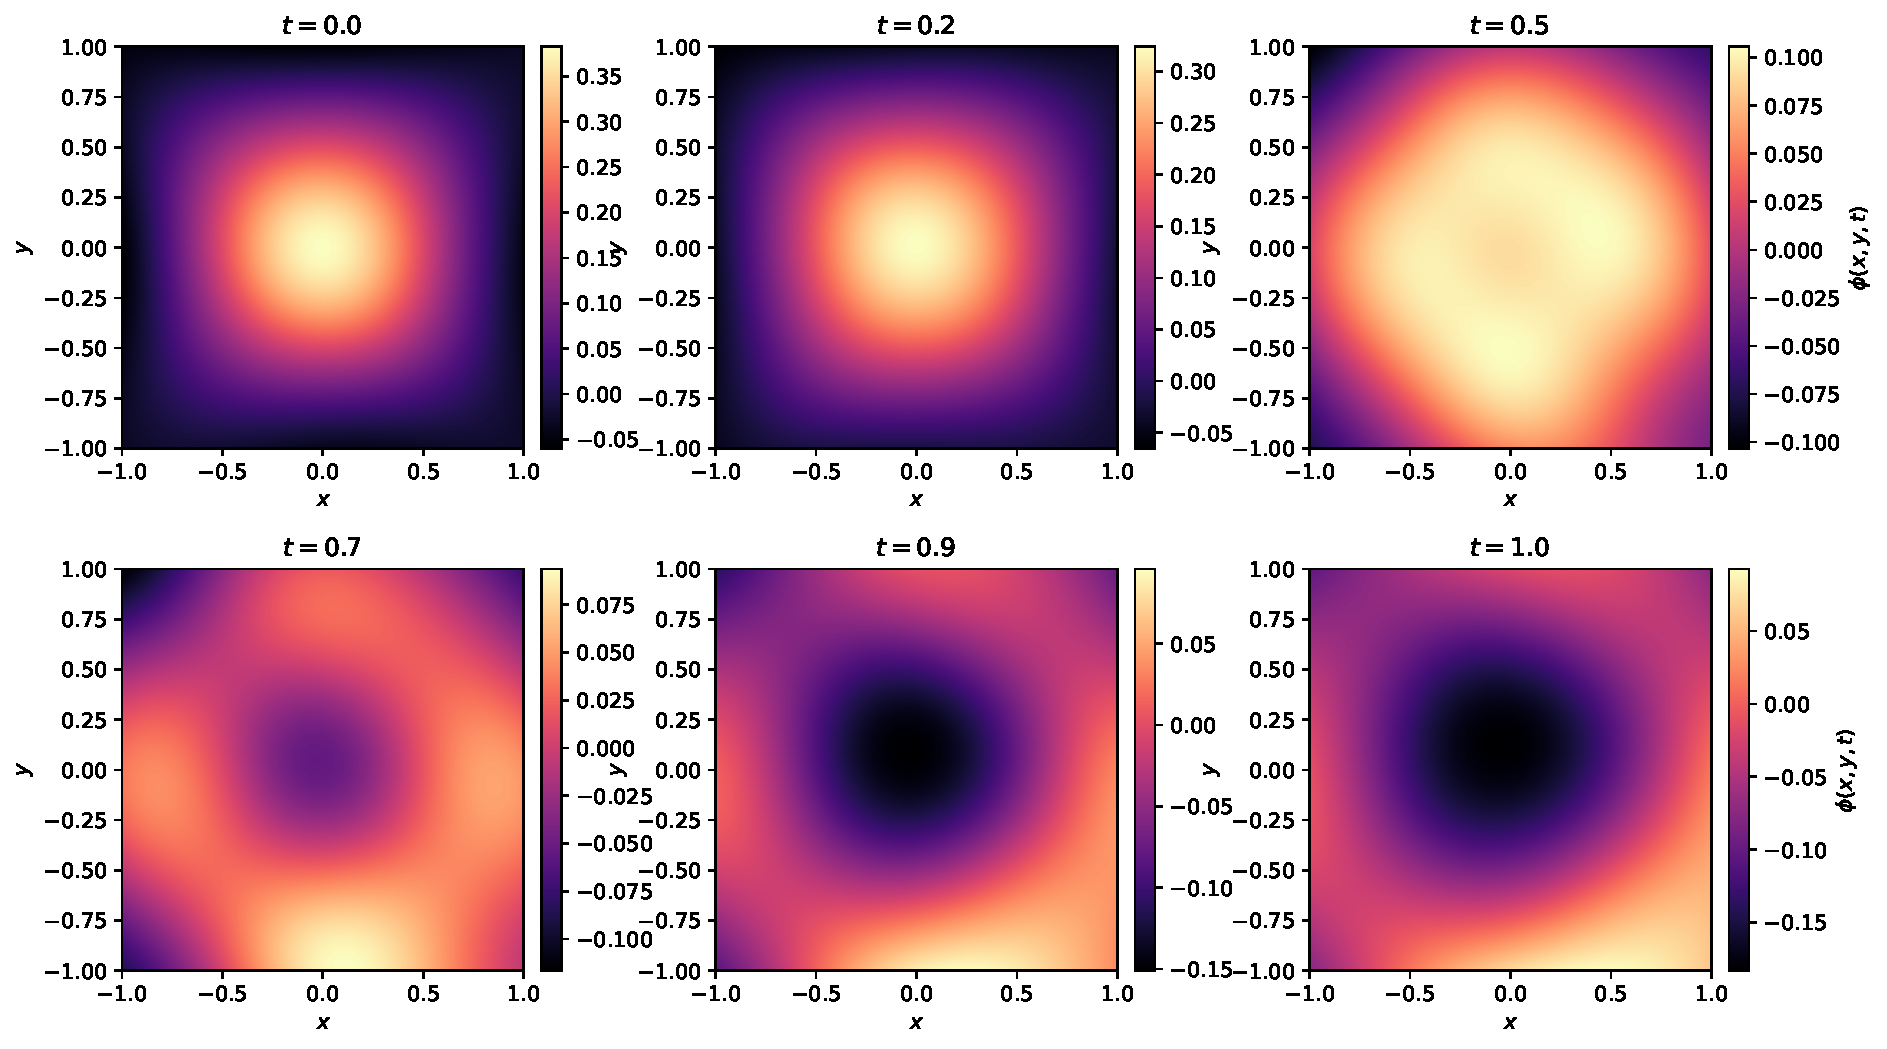
\includegraphics[width=0.95\textwidth]{examples/wave_field_eq.pdf}
    \caption[Solution for the nonlinear field equation]{\label{fig:field-pinn}
    Snapshots of the scalar field $\phi(x,y,t)$ at different times. 
    The nonlinear self-interaction generates ring-shaped wavefronts that propagate radially outward from the center, illustrating the nontrivial dynamics captured by the PINN.
    }
\end{figure}

These examples illustrate how physics-informed neural networks provide a unified and flexible framework for solving both linear and nonlinear differential equations, serving as a foundation for more advanced applications in complex physical systems.
% ============================================================
% ============================================================
\section{Summary}
\label{sec:dl_summary}

In this chapter, we have introduced the fundamental concepts required to understand and implement deep learning models within a rigorous mathematical framework. Beginning with the general formulation of learning problems in terms of tasks, experience, and performance measures, we established the conceptual foundations of machine learning and its specialization into deep learning architectures.

We reviewed the structure of artificial neural networks, including fully connected and convolutional layers, and discussed the role of activation functions in enabling nonlinear representation learning. The training process was formulated as a high-dimensional optimization problem, where backpropagation and gradient-based methods allow efficient parameter updates. Particular emphasis was placed on the interpretation of loss functions, since they define the objective that guides the learning dynamics.

The chapter culminated with the introduction of Physics-Informed Neural Networks, which extend conventional data-driven models by incorporating physical constraints directly into the training objective. By embedding differential equations, boundary conditions, and structural properties into the loss function, PINNs restrict the hypothesis space to physically admissible solutions. This approach enables accurate modeling of complex dynamical systems while reducing the dependence on large datasets.

Through the examples of the one-dimensional wave equation and the nonlinear Klein--Gordon equation in $(2+1)$ dimensions, we demonstrated how deep learning architectures can approximate both linear and nonlinear field dynamics. These case studies illustrate the capacity of physics-informed models to capture intricate spatiotemporal behavior while maintaining consistency with governing physical laws.

The framework developed in this chapter serves as the methodological foundation for the subsequent applications presented in this thesis, where physics-informed deep learning is employed to address advanced problems in quantum information and quantum dynamics.